\section{Observational background and basic assumptions}

\subsection{Introduction}

A star to be a star must satify two conditions:
\begin{itemize}
    \item It is bound by self-gravity (hence spherically symetric)
    \item It radiates energy from an internal source
\end{itemize}

Hence the end of a star happens when one of these conditions fails: the star either isin't bound by its own gravity, and thus breaks up and scatters material, or it doesn't produce energy internally, meaning it's nuclear fuel exhausts. Most stars end their lives in a combination of these two. 

Primary characteristic that can be measured is the \textit{apparent brightness} $I_{\rm obs}$ - is the flux of stars radiation (power over area), note that it's apparent since it depends on the distance to the observer. The power (energy per time) which radiated by a star is called \textit{luminosity} $L$, so

\begin{equation*}
    I_{\rm obs} = \frac{L}{4 \pi d^2} 
\end{equation*}

where $d$ is the distance to the observer. The effective temperature of a star $T_{\rm eff}$ is thus defined as the temperature of a blackbody. This is an approximation for the star's outermost layer - \textit{photosphere} (bulk of the emmited radiation comes from here).

\begin{equation*}
    \sigma T^4_{\rm eff} = \frac{L}{4 \pi R^2}
\end{equation*}

where $\sigma$ is the Stefan-Boltzman constant. According to Wein's law the maximum radiation wavelength $\lambda_{\max}$ is given by

\begin{equation*}
    \lambda_{\rm max} T = {\rm const}
\end{equation*}

Based on evidence there are some axioms that can be added to the general definition of a star

\begin{itemize}
    \item \textbf{Isolation} A single star may be considered isolated in empty space. Hence, initial conditions will exclusively determine it's evolution.
    \item \textbf{Uniform initial composition}. There is little difference in the initial composition of stars, of which the abundance of heavy elements within a star have the biggest influence, which is negligable compared to hydrogen and helium. The fate of the star is then solely depentend upon its initial mass $M$.
    \item \textbf{Spherical Symtry} In vast majority of the cases the rotation of a star or it's magnetic field are not strong enough to loose spherical symetry. Therefore, the physical properties of a star change with just the radius $r$.
    \begin{equation*}
        dm = \rho 4 \pi r^2 dr \quad \Rightarrow \quad m(r) = \int_0^r 4 \pi r^2 \rho(r) dr
    \end{equation*}
\end{itemize}


\begin{center}
    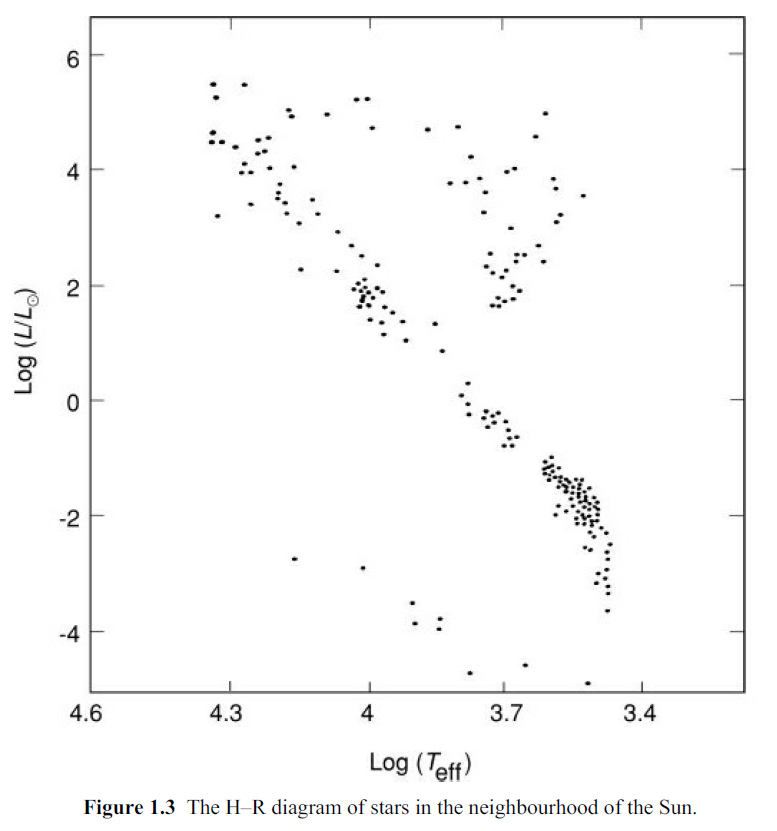
\includegraphics[width=200pt]{images/hr diagram.png}
    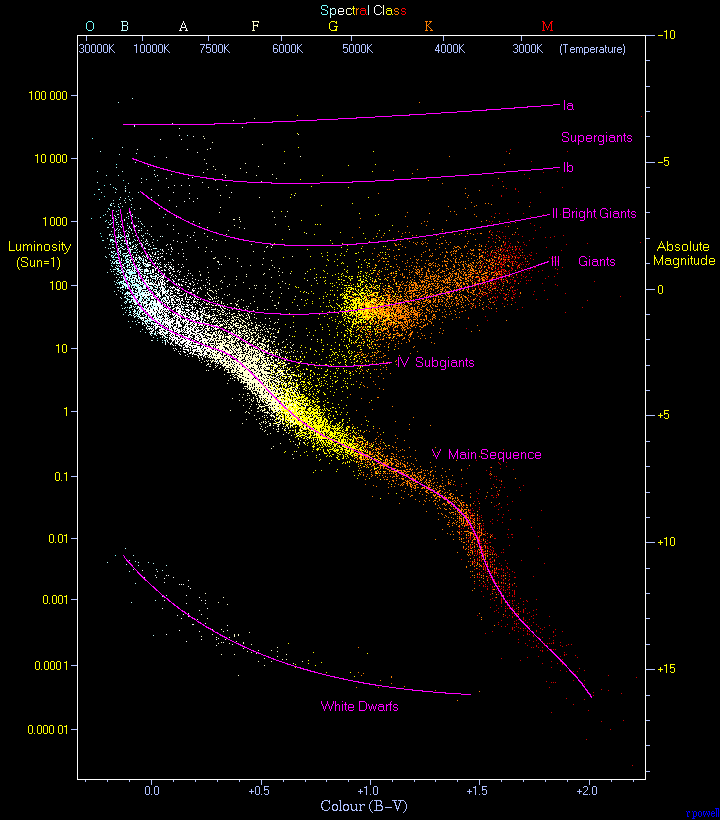
\includegraphics[width=200pt]{images/HRDiagram.png}
\end{center}

The thin strip in the middle is called \textbf{the main sequence} which corresponds stars called \textbf{main sequence stars}. The right blob above the main sequence (has the same or lower $T_{\rm eff}$ at the same $L$) have their spectrum shifter toward the longer wavelengths with a reddish colour. According to equations higher $L$ and lower $T_{\rm eff}$ implies a large radius. Such stars are called \textbf{red giants}. Their redii may attain several hundred solar radii.

Conversely, on the lower left corner are stars with low luminosities and high effective temperatures. Thus they have small radius and a bluish-white colour. They are accordingly named \textbf{white dwarfs}. Their radii are about the size of Earth's but they have the mass of the sun.

From the axioms we know that initial conditions (mass and age) are the main differentiators. Hence there are two ways to interpret HR diagram: either the stars in the diagram represent stars at different ages, thus allowing us to draw a line and seeing how the star evolves, or it's properties (Luminosity and Surface temperature) are highly dependent on mass. In general, we can conclude that being outside the main sequence is determined by age, while the location \textit{in main sequence} depends on mass. Note that the hotter the star in the main sequence the more massive it is. In addition, since high/low mass stars burn fuel way faster/slower, their lifetimes in main sequnce are shorter/longer. Hence the lower part of the main sequence (low temperature and mass) is basically constantly populated. In fact, there is a power-law dependence of main-sequence stars

\begin{equation*}
    L \propto M^{\nu} \quad \frac{L}{L_{\odot}} = \left( \frac{M}{M_{\odot}} \right)
\end{equation*}

\begin{center}
    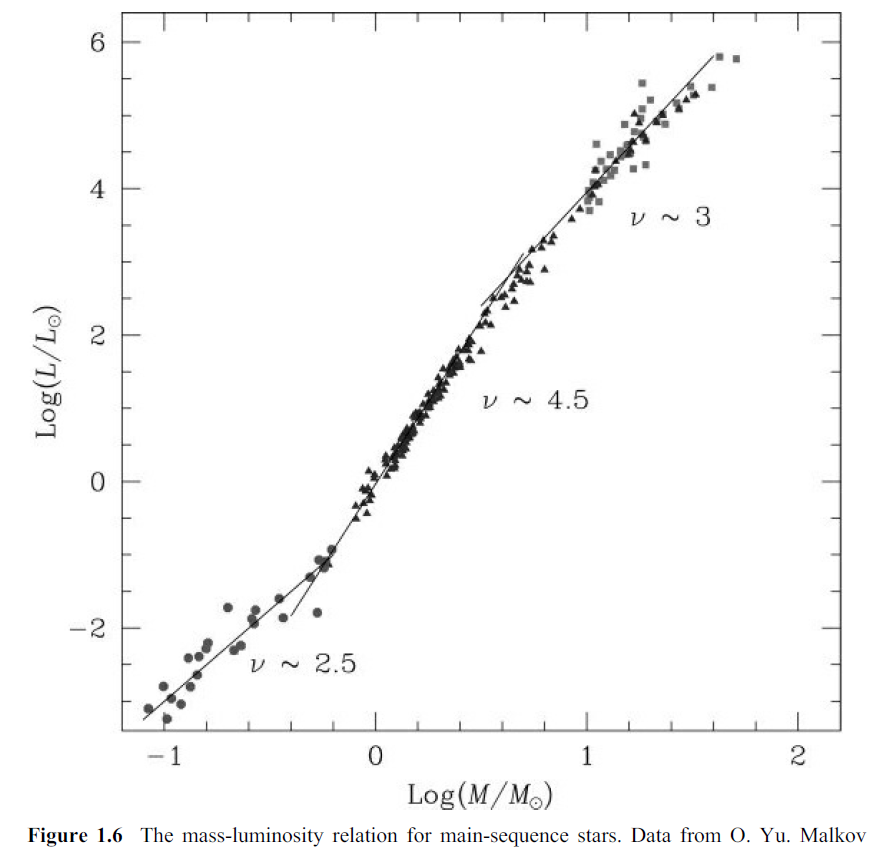
\includegraphics[width=200pt]{images/luminosity mass diagram.png}
\end{center}